\textbf{\underline{OZ 9 - Wisselstroomkringen - Oefening 3:}}
\vspace{0.5cm}

In de transformator is de weerstand in de belastingskring $R_L = 50.0 \ \Omega$. De verhouding van de windingen $\tfrac{N_1}{N_2} = \tfrac{5}{2}$, en de bronspanning is $80.0 \ \text{V}$ (rms). Als een voltmeter een belasting meet van $25.0 \ \text{V}$ (rms), wat is dan de bronweerstand $R_s$?

% \begin{enumerate}[(a)]
%     \item #
% \end{enumerate}

\begin{center}
    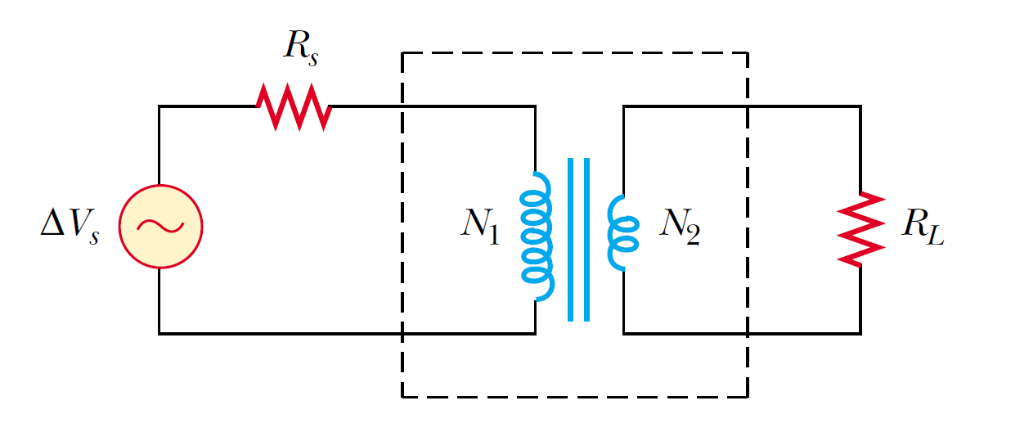
\includegraphics[scale = 0.4]{oz09/resources/Oz9Oef3.png}
\end{center}

\begin{description}[labelwidth=1.5cm, leftmargin=!]
    \item[Geg. :]   
    \item[Gevr. :] 
    \item[Opl. :]   
\end{description}

\vspace{1cm}